\documentclass{article}
\usepackage{amsmath}
\usepackage{graphicx}
\usepackage{geometry}
\usepackage{booktabs}

\usepackage{geometry}
\geometry{hmargin=2.5cm,vmargin=1.5cm}

\title{Modélisation de l'Accélération Libre des Véhicules}
\author{Nouni2}
\date{Juillet 2024}

\begin{document}

\maketitle


\section{Introduction}
L'accélération libre est un concept essentiel dans la modélisation du trafic routier. Dans ce contexte, l'accélération libre désigne l'accélération qu'un véhicule effectue pour atteindre une vitesse donnée \(v_{\text{lim}}\) en ignorant tout le trafic extérieur ainsi que les caractéristiques du terrain. En d'autres termes, il s'agit de l'accélération dans des conditions idéales de route et de trafic, où un véhicule accélère pour atteindre une vitesse cible sans être influencé par des facteurs externes tels que d'autres véhicules, des pentes ou des conditions météorologiques.

L'étude de l'accélération libre permet de comprendre comment les véhicules atteignent leurs vitesses cibles dans des scénarios optimaux. Cela fournit une base de référence pour évaluer les performances des véhicules et les comportements de conduite, ainsi que pour calibrer les modèles de simulation de trafic prenant en compte des conditions plus complexes.

\section{Distribution de la Vitesse}

L'objectif de cette section est de modéliser la distribution des vitesses des véhicules sur une route limitée par une vitesse maximale \(v_{\text{max}}\). Idéalement, tous les véhicules accéléreraient uniformément pour atteindre exactement cette vitesse, mais en pratique, ce n'est jamais le cas. Certains véhicules dépassent même cette limite, ce qui entraîne une distribution autour de \(v_{\text{max}}\). 

Après plusieurs recherches et l'exploration de différentes distributions telles que la loi log-normale, nous avons retenu la distribution de Pareto inversée. Cette distribution est particulièrement adaptée car elle permet de modéliser une concentration des vitesses autour de \(v_{\text{max}}\) avec une décroissance après cette limite. La distribution de Pareto ordinaire est définie comme suit :

\[ 
f(x; \alpha, x_m) = \begin{cases} 
\frac{\alpha x_m^\alpha}{x^{\alpha+1}} & \text{pour } x \geq x_m, \\
0 & \text{pour } x < x_m.
\end{cases} 
\]

Pour obtenir la forme souhaitée, nous avons effectué un changement de variable \(u = v_{\text{param}} - v\), où \(v_{\text{param}}\) est un paramètre dépendant de la vitesse maximale \(v_{\text{max}}\). Ce changement de variable permet d'ajuster la courbe autour de \(v_{\text{max}}\), car \(v_{\text{max}} - v_{\text{param}}\) limite le domaine de définition de la fonction à \([0, v_{\text{max}}]\), ce qui permet de prendre en compte les valeurs supérieures à \(v_{\text{max}}\).

Ainsi, après étude de la fonction, la forme retenue est :

\[ 
\varphi(v; \alpha, \beta) = \frac{\alpha \beta^\alpha}{(v_{\text{param}} - v)^{\alpha + 1}} \exp\left(-\beta (v_{\text{param}} - v)^{-\alpha}\right).
\]

Il reste alors à déterminer les valeurs des paramètres. Nous cherchons à ajuster le maximum de la courbe autour de \(v_{\text{max}}\), ce qui impose que \(\partial \varphi / \partial v_{\text{param}} (v_{\text{max}}) = 0\). La dérivée de \(\varphi\) est donnée par :

\[ 
\frac{\partial \varphi}{\partial v_{\text{param}}} = \alpha \beta^\alpha (v_{\text{param}} - v)^{-2(\alpha + 1)} \left( -\exp\left(-\beta (v_{\text{param}} - v)^{-\alpha}\right) \right) \left( \alpha ((v_{\text{param}} - v)^{-\alpha} - \beta) + (v_{\text{param}} - v)^{-\alpha} \right).
\]

En résolvant l'équation \(\partial \varphi / \partial v_{\text{param}} = 0\), nous trouvons :

\[ 
v_{\text{param}} = v_{\text{max}} - \left( \frac{\beta \alpha}{\alpha + 1} \right)^{\frac{1}{\alpha}}.
\]

Cependant, un facteur d'agressivité \(k\) (entre 0 et 1) a été rajouté et l'équation finale de \(v_{\text{param}}\) est donc :

\[ 
v_{\text{param}} = v_{\text{max}} \times (1.05 + 0.03 \times k) - \left( \frac{\beta \alpha}{\alpha + 1} \right)^{\frac{1}{\alpha}}.
\]

La valeur de \(\alpha\) a été choisie empiriquement, tandis que \(\beta\) sera discutée plus tard. La figure ci-dessous montre les distributions de vitesses pour différentes valeurs de \(\beta\).

\begin{figure}[h!]
    \centering
    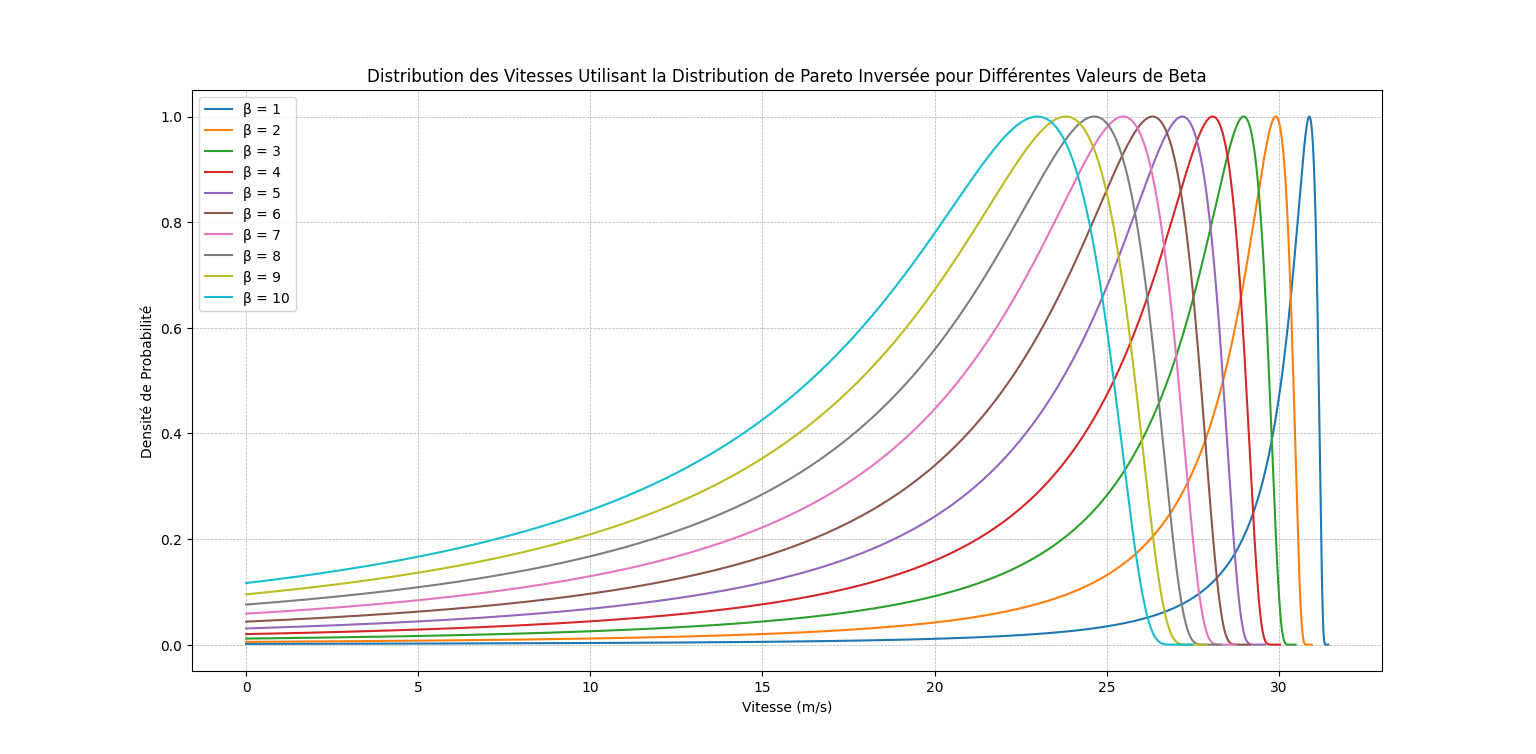
\includegraphics[width=\linewidth]{Free Speed Distribution.png}
    \caption{Distributions des vitesses normalisée par \( \displaystyle \max_{v \in [0, v_{\text{param}}]}(\varphi) \) pour différentes valeurs de \(\beta\) et \( \alpha = 1.4 \).}
    \label{fig:pareto_distributions}
\end{figure}



\section{Choix de \(\beta\) et Attribution des Vitesses}

Pour modéliser la distribution des vitesses des véhicules, nous avons introduit un paramètre appelé ratio, noté \(r\). Ce ratio représente la proportion de la surface de la courbe \(\varphi(v)\) autour de \(v_{\text{max}}\) dans un intervalle \(v_{\text{interval}}\) (pris à 10\% dans les simulations) par rapport à la surface totale de la courbe. Ce paramètre permet de contrôler l'étalement des vitesses autour de \(v_{\text{max}}\). Plus \(r\) est proche de 1, plus les vitesses sont concentrées autour de \(v_{\text{max}}\), et vice versa.

\subsection{Fonction de Distribution Cumulative}

Pour attribuer une vitesse à chaque véhicule, nous définissons la fonction de distribution cumulative \(F(v)\) comme l'intégrale de la densité de probabilité \(\varphi(v)\) :

\[
F(v) = \int_0^v \varphi(u) \, du
\]

Nous normalisons ensuite cette fonction par sa valeur maximale pour obtenir \(\tilde{F}(v)\) entre 0 et 1. Pour chaque véhicule, nous tirons un \(u\) aléatoire entre 0 et 1 et lui associons une vitesse \(v\) telle que \(\tilde{F}(v) = u\). La résolution se fait numériquement, permettant d'attribuer une vitesse à chaque véhicule en fonction de la distribution définie.

\subsection{Détermination de \(\beta\)}

Pour ajuster la distribution des vitesses, nous devons déterminer la valeur de \(\beta\) en fonction de \(v_{\text{max}}\) et du ratio \(r\). Nous avons utilisé une forêt aléatoire pour effectuer cette régression. Voici les étapes détaillées du processus :

1. \textbf{Calcul du ratio $r$:} 
   Pour chaque paire de valeurs \((v_{\text{max}}, r)\), nous avons calculé le ratio des véhicules dont les vitesses se situent dans l'intervalle \(v_{\text{max}} \pm v_{\text{interval}}\) en utilisant la fonction de densité de probabilité \(\varphi(v; \alpha, \beta)\). Le calcul du ratio est effectué à l'aide de la fonction de répartition cumulative normalisée \(\tilde{F}(v)\).

2. \textbf{Génération des Données} :
   Nous avons généré des données pour différentes valeurs de \(v_{\text{max}}\) et \(r\), et calculé la valeur optimale de \(\beta\) pour chaque paire en utilisant une méthode de minimisation numérique. Cette méthode cherche à minimiser la différence entre le ratio calculé et le ratio cible \(r\).

3. \textbf{Entraînement du Modèle} :
Nous avons utilisé une forêt aléatoire pour entraîner un modèle de régression afin de prédire \(\beta\) en fonction de \(v_{\text{max}}\) et \(r\). 

Une forêt aléatoire est un ensemble d'arbres de décision utilisé pour des tâches de régression et de classification. Elle fonctionne en construisant plusieurs arbres de décision lors de l'entraînement et en produisant la moyenne des prédictions de chaque arbre pour améliorer la précision et contrôler le sur-apprentissage.

La figure ci-dessous montre les prédictions du modèle par rapport aux données réelles pour différentes valeurs de \(\beta\) en fonction de \(v_{\text{max}}\) et \(r\).

\begin{figure}[h!]
 \centering
 \includegraphics[width=\textwidth]{Foret aléatoire beta.png}
 \caption{Modèle de forêt aléatoire pour \(\beta\).}
 \label{fig:foret_aleatoire_beta}
\end{figure}

4. \textbf{Prédiction des Valeurs de \(\beta\)} :
   Le modèle entraîné permet de prédire la valeur de \(\beta\) pour toute paire de valeurs \((v_{\text{max}}, r)\), assurant ainsi une distribution des vitesses conforme aux spécifications de la simulation.

Ce processus permet de déterminer de manière efficace et précise les valeurs de \(\beta\) pour ajuster la distribution des vitesses des véhicules autour de \(v_{\text{max}}\), en tenant compte de l'étalement souhaité défini par le ratio \(r\).


\newpage

\section{Modélisation de l'Accélération Libre}

L'accélération libre d'un véhicule, c'est-à-dire l'accélération qu'il effectue pour atteindre une vitesse cible en l'absence de trafic et de conditions de route adverses, est un aspect crucial du réalisme de notre simulation. Modéliser cette accélération de manière précise nécessite de prendre en compte la dépendance de l'accélération à la vitesse cible.

L'approche simple consistant à diviser la vitesse cible par un temps d'accélération constant n'est pas suffisante car elle ne capture pas la variation de l'accélération avec la vitesse. Par conséquent, nous introduisons le temps d'accélération par unité de vitesse, noté \(t_{\text{acc\_per\_unit\_v}}\), qui représente le temps nécessaire pour accélérer d'une unité de vitesse.

Deux modèles ont été envisagés pour modéliser \(t_{\text{acc\_per\_unit\_v}}\) :

1. Modèle logarithmique :
   \[
   t_{\text{acc\_per\_unit\_v}} = t_0 \log\left(1 + \frac{v}{v_{\text{ref}}}\right)
   \]

2. Modèle racine carrée :
   \[
   t_{\text{acc\_per\_unit\_v}} = t_0 \left(1 + \sqrt{\frac{v}{v_{\text{ref}}}}\right)
   \]

Après analyse, nous avons retenu le modèle racine carrée. Ce modèle a été ajusté pour correspondre à des points de référence. Les paramètres retenus sont :
\[
t_0 = 0.15 \, \text{s/km/h}
\]
\[
v_{\text{ref}} = 16.26 \, \text{km/h}
\]

La figure ci-dessous illustre le modèle racine carrée pour \(t_{\text{acc\_per\_unit\_v}}\) :

\begin{figure}[h!]
    \centering
    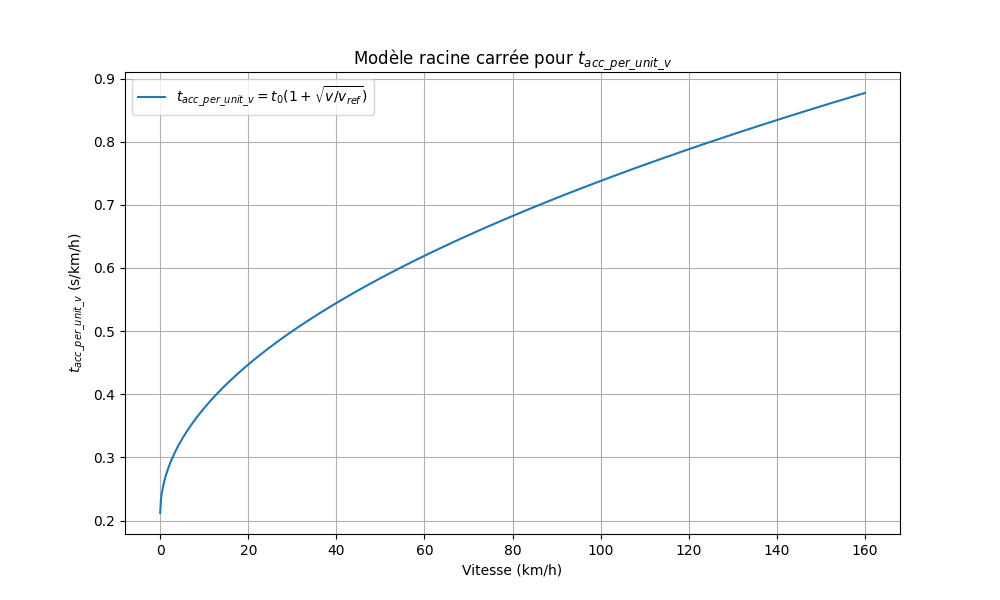
\includegraphics[width=\textwidth]{sqrt model.png}
    \caption{Modèle racine carrée pour \(t_{\text{acc\_per\_unit\_v}}\).}
    \label{fig:sqrt_model}
\end{figure}

\section{Calcul de l'Accélération Libre}
Pour chaque véhicule, nous modélisons le temps d'accélération par unité de vitesse en utilisant une distribution gaussienne avec une moyenne \(t_0\) et un écart-type de \(0.1 \cdot t_0\). Ce temps d'accélération par unité de vitesse, noté \(t_{\text{acc\_per\_unit\_v}}\), permet de prendre en compte la variabilité des conducteurs dans notre simulation.

L'accélération nécessaire pour atteindre la vitesse cible \(v_{\text{lim}}\) à partir de la vitesse initiale \(v_i\) est donnée par :
\[
a = \frac{v_{\text{lim}} - v_i}{t_{\text{acc\_per\_unit\_v}} \cdot v_{\text{lim}}}
\]


La figure ci-dessous montre la courbe du modèle racine carrée pour \(t_{\text{acc\_per\_unit\_v}}\) en fonction de la vitesse, ainsi que l'accélération moyenne en fonction de la vitesse maximale :

\begin{figure}[h!]
    \centering
    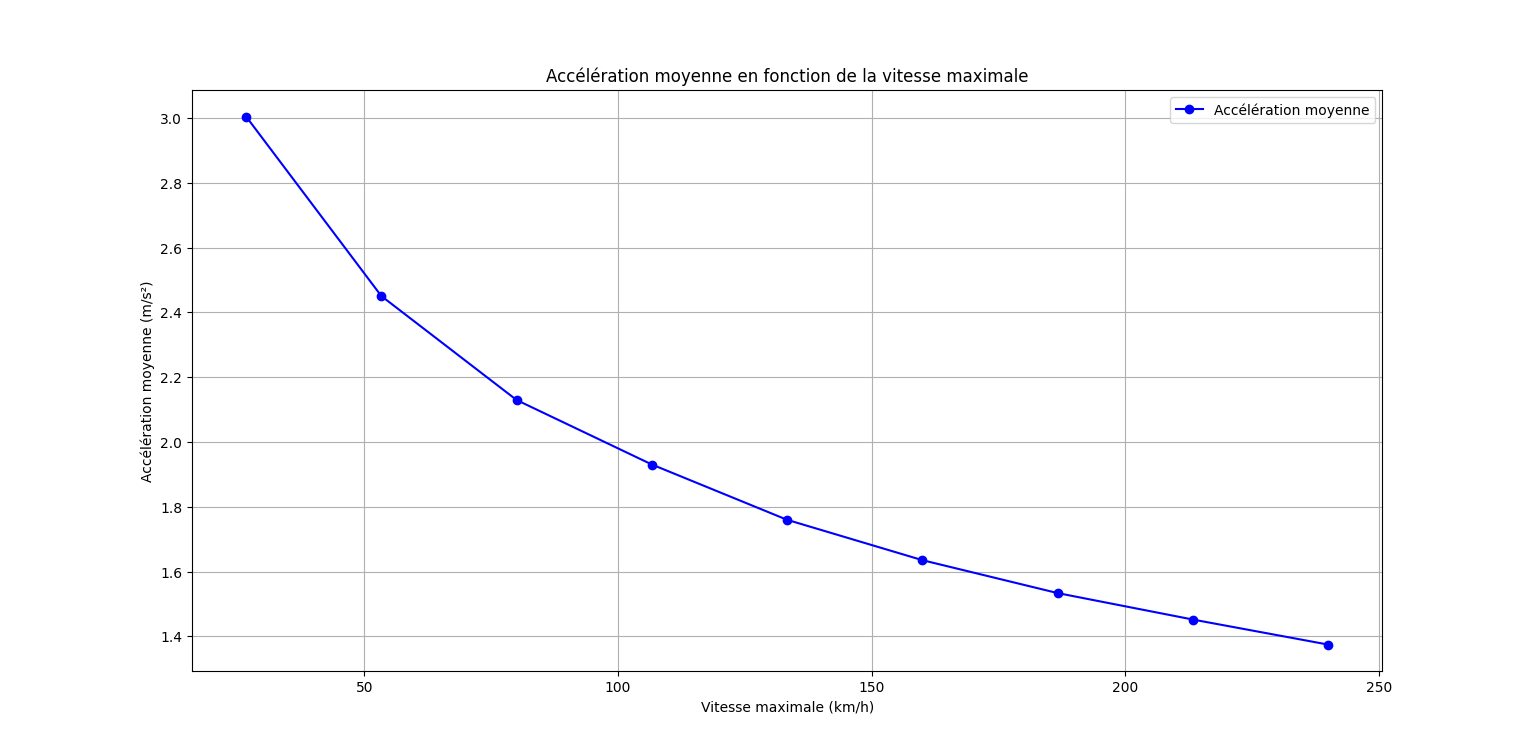
\includegraphics[width=\textwidth]{Free acceleration.png}
    \caption{Accélération moyenne en fonction de la vitesse maximale.}
    \label{fig:free_acceleration}
\end{figure}

\end{document}
